\documentclass{article}
\usepackage[french]{babel}
\usepackage[utf8]{inputenc}
\usepackage{graphicx}
\usepackage{geometry}
\usepackage{subfig}
\usepackage{listings}
\usepackage[T1]{fontenc}
\usepackage{courier}
\usepackage[colorlinks=true]{hyperref}

\hypersetup{
    linktoc=all,
    linkcolor=blue
}
\setlength{\parindent}{1cm}
\graphicspath{ {tex/files/} }

\title{Rapport Projet S6 - IMPERATIVE}
\author{Romain PIERRE, Mathys MONELLO, Ilyes BECHOUAL, Yannis YOASSI PATIPE}
\date{Mai 2023}

\makeatletter
\let\mytitle\@title
\let\myauthor\@author
\let\mydate\@date
\makeatother

\begin{document}

\lstset{language=C, frame=single, basicstyle=\ttfamily, tabsize=4}

\begin{titlepage}
    \centering
    \vspace*{0.5 cm}
    
\includegraphics[width=5cm]{logo.jpg}\\[1.0 cm]
    \rule{\linewidth}{0.2 mm} \\[0.4 cm]
    \huge\textbf{\mytitle}\\
    \rule{\linewidth}{0.2 mm} \\[1.5 cm]  
    \LARGE\myauthor\\[1.0 cm]
    \large\textbf{\mydate}\\[2 cm]
    \begin{center}
        \huge
        "AMAZONS"
    \end{center}

    \vspace{4cm}
    \begin{center}
    EI6PR105 Projet de programmation impérative
    \\Département Informatique
    \\S6 - Année 2022/2023
    \end{center}
 \end{titlepage}

\tableofcontents

\newpage
\section{Introduction}
Le jeu \textbf{Amazons} est un jeu de stratégie sur plateau, et est l'objet de notre projet de programmation impérative du semestre 6. Le but de ce projet est de produire un code qui met en place une stratégie pour chaque joueur afin qu'il puisse jouer d'eux même, en respectant les règles du jeu. Il faut aussi pour cela, créer un serveur qui permet la communication de certaines données aux joueurs et de modéliser le jeu. Pour créer les jeux, nous allons devoir modéliser les plateaux en les manipulant sous forme de graphes, afin de permettre aux joueurs de jouer sur plusieurs plateaux sans prendre en compte leur forme. Nous utiliserons de nouvelles bibliothèques comme \textbf{GSL} et \textbf{DLopen} par exemple pour optimiser la compléxité de certaines fonctions et permettre le chargement dynamique des clients.

\vspace{1cm}
\section{Compte-rendu}
Lors de ce projet, nous avons créé notre propre serveur, ainsi que deux joueurs ayant leur propre stratégie. Nous n'avons réalisé que les graphes carré et grille pour lesquels nous avons réalisé des tests afin d'observer si les valeurs des matrices d'adjacences étaient correctes.
\\La stratégie du joueur nommé \textit{Georges} consiste à prendre possession du centre du plateau afin d'attaquer les extrémités du plateau pour réduire l'espace de jeu le plus rapidement possible, mais aussi pour avoir un large éventail de possibilités pour tirer une flèche près de l'adversaire et réduire son espace de jeu et ses possibilités de déplacement ou d'attaque.
\\La stratégie du second joueur nommé \textit{David} est une stratégie qui s'articule en deux points. Premièrement, il s'agit de privilégier les mouvements vers les zones libres afin de maximiser la liberté et les possibilités de mouvement des reines. Deuxièmement, il s'agit de privilégier les attaques à proximité des reines adverses pour réduire leur possibilité de mouvement et ainsi les forcer à la faute.
\\Nous avons majoritairement testé les fonctions qui servent à jouer et les fonctions utilitaires du serveur.

\newpage
\section{Architecture du projet}
Cette section présente les choix d'architecture qui ont été fait pour ce projet.

\subsection{Dépendances}
Notre projet se décompose en 9 fichiers:

\begin{itemize}
    \item \textbf{player} contient toutes les spécifications des clients.
    \item \textbf{game} contient toutes les fonctions utilitaires liées au jeu.
    \item \textbf{move} contient la structure \textit{move\_t} qui assure l'interopérabilité entre les clients et le serveur pour l'échange de coup.
    \item \textbf{graph} contient les spécifications des graphes et leurs fonctions associées.
    \item \textbf{dir} contient l'énumération \textit{dir\_t} des 8 directions possibles.
    \item \textbf{sever\_aux} contient les fonctions utilitaires propres au serveur.
    \item \textbf{server} est le serveur et le "main" du projet.
    \item \textbf{David} et \textbf{Georges} sont les 2 clients du projet. Ils contiennent leur propre stratégie et leurs informations.
\end{itemize}

\begin{figure}[!h]
    \centering
    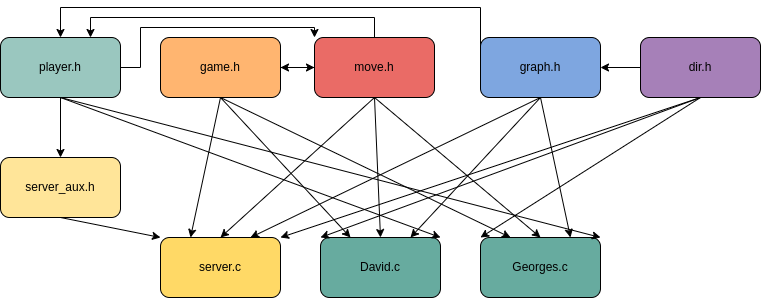
\includegraphics[width=12cm]{diag_c.drawio.png}
    \caption{Graphe des dépendances}
    \label{fig:depend}
\end{figure}

\subsection{Programmation modulaire}
L’intérêt premier de ce choix d’architecture est d’avoir un code modulaire. En effet, en regroupant les sous-problèmes en fichiers distincts, il est plus facile de maintenir le projet ou l’améliorer. Il
suffit de respecter l’interface fixée et on peut ensuite travailler librement au sein même du fichier
sans altérer le reste du projet. De même, il n’est pas nécessaire d’avoir tous le projet en tête, et la
simple connaissance du fichier en question est suffisante pour travailler dessus.
Ainsi, la programmation modulaire facilite la modification du code et limite les bugs qui pourraient se généraliser à l’ensemble du projet, en contenant l’information au sein d’un même fichier. Il est
donc plus facile de se repérer et de collaborer.

\newpage
\section{Stockage des reines}
\label{tabqueen}

Pour stocker les informations sur les reines, nous avons décidé d'implémenter deux façons avec leur avantage et leur inconvénient.

\subsection{Tableau des indices}
\label{petittab}
La première implémentation est une paire de pointeur vers \textbf{num\_player} tableaux de taille \textbf{num\_queen} nommée \textbf{queens\_idx}.  Les tableaux contiennent les indices (numéro de sommet) des reines des joueurs de la partie (dans le tableau du joueur correspondant). Il y a un tableau de reine par joueur. 
\vspace{0.5cm}

Ce tableau permet d'obtenir en temps linéaire la position des reines, ce qui permet un gain en complexité pour itérer sur les reines car $\textit{num\_queen} \ll \textit{num\_vertices}$. C'est ce tableau que le serveur envoie aux clients, par spécification du sujet. 
\vspace{0.5cm}

L'inconvénient est que pour vérifier la présence d'une reine sur un indice spécifique il faut itérer sur tout le tableau. Cette action étant nécessaire souvent, on se donne une deuxième implémention permettant un temps constant.

\subsection{Tableau des sommets}
\label{grandtab}
La deuxième implémentation est une paire de pointeur vers \textbf{num\_player} tableaux de taille \textbf{num\_vertices} nommée \textbf{queens}.  Les tableaux contiennent des 0 partout sauf aux indices \textit{position d'une reine} où ils contiennent un 1. Il y a un tableau de reine par joueur. 
\vspace{0.5cm}

Ce tableau permet de savoir en temps constant si une reine est présente sur un sommet. Cela permet un gain en complexité pour itérer sur les sommets, notamment lorsqu'on liste les mouvements possibles en vérifiant rapidement qu'une reine ne bloque pas une direction. Ce tableau n'est pas envoyé par le serveur aux clients, il est reconstruit par la fonction \textit{initialize()} grâce au tableau d'indices \textbf{queens\_idx} de la section \ref{petittab} (voir section \ref{playerdata}). La figure \ref{fig:queen} montre un exemple de ces deux implémentations pour un joueur.

\begin{figure}[!h]
    \centering
    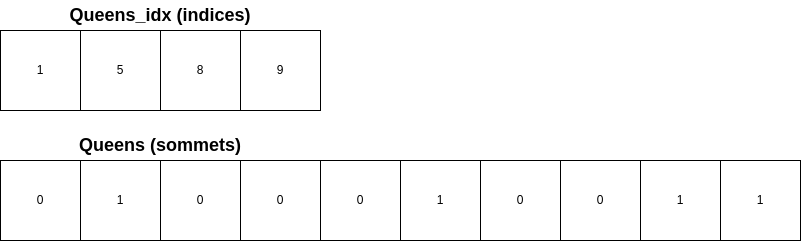
\includegraphics[width=12cm]{queen.drawio.png}
    \caption{Exemple des deux implémentations pour un joueur}
    \label{fig:queen}
\end{figure}

\newpage
\section{Graphe}
\label{graph}
Dans cette partie, nous allons parler de l'implémentation du jeu, du type de graphes que nous avons utilisé et de la manière dont nous avons pu les optimiser.

\subsection{Implémentation du jeu}
L'implémentation de ce jeu se réalise sous la forme de graphe, c'est-à-dire qu'on considère qu'une case est un sommet et qu'un déplacement n'est possible qu'au travers d'un arc. Les reines pouvant se déplacer dans toutes les directions en ligne droite, mais les arcs ne possédant pas tous le même poids, le graphe est donc un graphe orienté multiple. L'utilisation de graphe permet aussi l'utilisation d'une matrice d'adjacence pour mettre en évidence les liaisons entre les sommets et ainsi savoir où l'on peut se rendre à l'aide du sommet source. Cette matrice est plutôt simple à lire car elle contient un coefficient $c_{i,j}$ nul lorsqu'un déplacement entre deux sommets $i$ et $j$ est impossible et un coefficient non nul lorsque le déplacement est possible. 

\subsection{Types de graphes}
Lors de ce projet, nous avons implémenté les graphes \textbf{carrés}, \textbf{grilles} et \textbf{donuts}. Ils se distinguent par le nombre de directions dans lesquels peut se déplacer la reine, respectivement 8 et 4 directions (cardinales) et par leur structure pleine ou non. Ainsi, pour
construire les graphes non pleins, nous construisons d'abord les graphe \textbf{carré} et nous désactivons les sommets dans les vides en supprimant leurs arcs. Puis nous créons un nouveau graphe de taille \textit{nombre de sommet}, en écrivant uniquement les valeurs non nulles. Ainsi les graphes sont bien encodés sous forme d'une matrice d'adjacence creuse.
\subsection{Optimisation GSL - format CSR}
L'utilisation de matrice d'adjacence implique une complexité en $\Theta(n*m) $ avec $n$: le nombre de lignes de la matrice et $m$: le nombre de colonnes de la matrice. C'est pourquoi nous avons dû utiliser le format \textbf{CSR} de la bibliothèque GSL. Ce format permet de regrouper les informations importantes pour accéder aux éléments non nuls dans trois tableaux. Ainsi la complexité pour accéder à un élément non nul devient $\Theta(nnz*m)$ avec $nnz$: le nombre d'éléments non nuls dans la matrice d'adjacence du graphe. On utilise par exemple cette optimisation pour supprimer des arcs lorsqu'une flèche est tirée sur un sommet. En effet, nous connaissons déjà la ligne et la colonne de la matrice que nous devons modifier, ce qui nous permet d'itérer seulement sur les valeurs non nuls plutôt que sur l'ensemble des valeurs de la matrice. 
\newpage
\section{Serveur}
Le \textit{main} de notre projet est le fichier \textbf{server.c}. Il est le serveur au sens qu'il initie la partie, centralise l'information et gère les appels des clients (voir section \ref{client}) en étant l'intermédiaire.

\subsection{Spécification}
Le serveur suit la logique suivante :

\begin{enumerate}
    \item Récupérer les paramètres d'exécution avec \textit{getopt}.
    \item Charger les librairies dynamique avec \textit{DLopen} (voir section \ref{chargdyn}).
    \item Choisir le joueur qui commence.
    \item Initier le monde (voir section \ref{graph}).
    \item Initier les tableaux de reines (voir section \ref{tabqueen}).
    \item Envoyer les copies aux clients par mesure de sécurité (voir section \ref{secu}).
    \item Gérer la boucle de jeu.
    \item Vérifier la validité de chaque coup (voir section \ref{secu}).
    \item Déterminer le vainqueur.
    \item Libérer la mémoire (sauf copie).
    
\end{enumerate}

Le serveur doit donc imposer une interface avec les clients pour qu'ils puissent échanger avec lui. Ces spécifications sont débattues en section \ref{specclient}.

\subsection{Chargement dynamique}
\label{chargdyn}
Pour effectuer le chargement dynamique, nous avons stocké les pointeurs des fonctions de chaque client (voir section \ref{client}) dans un tableau de struct \textit{player\_t} de taille NUM\_PLAYER.
\vspace{0.5cm}

\noindent Voici le détail de cette structure de donnée :
\begin{lstlisting}
// Struct to contains all the function pointers for one player
struct player_t{
    void * lib;
    char const* (*get_player_name)(void);
    void (*initialize)(unsigned int player_id, struct graph_t* graph,
                    unsigned int num_queens, unsigned int** queens);
    struct move_t (*play)(struct move_t);
    void (*finalize)(void);
};

// Struct to contains all the player_t struct
struct players_t{
    struct player_t player[NUM_PLAYERS];
};
\end{lstlisting}

\noindent Ainsi le serveur peut appeler facilement les fonctions de chaque client en chargeant le struct \textit{player\_t} correspondant au  joueur courant.

\subsection{Sécurité}
\label{secu}

L'autre rôle majeur du serveur après l'orchestration de la partie, est de l'arbitrer. Pour cela le serveur a 2 tâches supplémentaires.

\subsubsection{Envoi de copies}

Avant le début de la partie, le serveur va devoir donner aux clients le monde sous forme de graphe et les tableaux de reine afin de leur permettre de pouvoir jouer des coups. Si le serveur décidait de donner directement les pointeurs vers son propre monde et ses propres tableaux de reine, cela voudrait dire que le client pourrait librement modifier les données de la partie et donc tricher et/ou corrompre la partie. Pour éviter cela nous allons cloisonner l'information pour le serveur et pour chaque client en la dupliquant. Ainsi le serveur va créer un nouveau monde et un nouveau tableau de reine pour chaque client, copier les informations actuelles à l'intérieur, et les envoyer au client à l'aide de la fonction \textit{initialize} (voir section \ref{client}). Alors, il sera impossible pour une entité de modifier directement les informations d'une autre.

\subsubsection{Vérification du coup}
\label{secumove}
À présent, un client ne peut modifier le monde ou les tableaux de reine qu'au travers de \textit{play} et de l'envoi d'un struct \textit{move\_t}. Mais cela ne prévient pas d'un coup illégal. le serveur doit donc à chaque coup, vérifier la validité du coup entrant avant de mettre à jour l'état du serveur et faire jouer l'autre joueur. Si un joueur joue un coup illégal, le serveur le disqualifiera et l'autre joueur sera déclaré gagnant.
\vspace{0.5cm}

Pour facilement vérifier les coups possibles, nous avons décider d'écrire une fonction qui les listes dans un struct \textit{set\_t}. Il suffit alors de vérifier que le coup joué appartient à ce set pour le qualifier de valide.
\vspace{0.5cm}

\begin{lstlisting}
struct set_t{
    unsigned int * idx;
    unsigned int len;
};
\end{lstlisting}

\newpage
\section{Clients}
\label{client}

Les joueurs de la partie sont appelés \textbf{clients}. Ce sont des bibliothèques dynamiques qui seront chargées par le serveur. Elles doivent respecter une interface imposée pour pouvoir discuter avec le serveur. 

\subsection{Spécification}
\label{specclient}

Le côté client suit la logique suivante :
\begin{enumerate}
    \item  S'identifier auprès du serveur avec \textit{get\_player\_name()}
    \item Récupérer et stocker les informations du serveur avec  \textit{initialize()}.
    \item Choisir un mouvement et prendre en compte le coup précédent avec \textit{play()}.
    \item Libérer la mémoire à la fin de la partie avec \textit{finalize()}.
\end{enumerate}

\subsection{Stockage des données de jeu}
\label{playerdata}
Pour stocker les informations venant du serveur nous avons créée une structure, la structure player\_data\_t :

\begin{lstlisting}
struct player_data_t {
    unsigned int player_id;
    unsigned int num_queens;
    struct graph_t * graph;
    int width;
    unsigned int * queens[NUM_PLAYERS];
    unsigned int * queens_idx[NUM_PLAYERS];
};
\end{lstlisting}
\vspace{0.5cm}

\noindent Nous avons choisi cette implémentation car elle nous permet de stocker les informations les plus utiles du serveur telles que le graphe, le nombre de reines, ou encore les tableaux de reine. Le tableau \textit{queen} "sur les sommets" est reconstruit dans \textit{initialize()} car seul \textit{queen\_idx} est envoyé par le serveur au travers de la fonction \textit{initialisze()}. Les informations sont rassemblées en une seule structure, ce qui facilite leur stockage en les rendant plus accessibles.

\newpage
\subsection{Stratégies}
Afin de savoir si la meilleure stratégie est l'attaque ou la défense, nous avons doté nos joueurs de stratégies distinctes. La première est une stratégie défensive et la seconde une stratégie plus offensive.

\subsubsection{Stratégie défensive}
La stratégie défensive vise à permettre aux reines d'attaquer l'adversaire tout en gardant un maximum de mobilité. Pour cela, nous avons implémenté trois \textbf{heuristiques} (deux pour le déplacement et une pour le tir de flèche) qui permettent de classer les différents coups possibles:
\begin{enumerate}
\item \underline{Déplacement d'une reine:}
\begin{itemize}
\item \textbf{Heuristique 1}: Cette première heuristique calcule le nombre de directions accessibles depuis une position donnée. Une position compte pour un point. 
\\Ex : Si la reine peut aller au \textit{Nord, Sud, Est et Ouest}, cela fait 4 points.
\item \textbf{Heuristique 2}: Cette heuristique calcule le nombre de mouvements simples (ou positions accessibles) à partir d'une position. \\Ex : Si la reine peut se déplacer 2 fois au \textit{Nord} et 4 fois au \textit{Sud}, cela fait 6 points.
\end{itemize}
\vspace{0.2cm}
Ces deux heuristiques ont le même esprit.En effet, elles sont là pour quantifier la liberté d'une position.
\item \underline{Tir de flèche}
\begin{itemize}
\item \textbf{Heuristique 3}: Cette heuristique est là pour favoriser les tirs de flèches à proximité des reines adverses. Ici, plus la flèche est proche d'une reine adverse, plus son score heuristique sera élevé (cela est possible car l'heuristique correspond à l'opposé de la valeur de la distance flèche-reine).
\\Ex : Si la flèche 1 est à une distance de 12 d'une reine et que la flèche 2 est à une distance 13 d'une reine, on aura :
\\h3(flèche 1) = - distance = -12  >  h3(flèche 2) = - distance = -13.
\end{itemize}
\end{enumerate}
En combinant ces heuristiques, on réussit à avoir une stratégie défensive cohérente. De plus dans cette stratégie nous faisons appel à une structure similaire à \textit{set\_t} de la section \ref{secumove} pour stocker la liste des mouvements possible, mais nous rajoutons un champ pour stocker en plus les directions. Cela est nécessaire pour les heuristiques de ce client.
\subsubsection{Stratégie du milieu}
La stratégie du milieu est une stratégie que nous qualifions d'offensive, elle consiste à prendre possession du milieu et à réduire la taille du plateau en tirant des flèches aux extrémités de ce dernier. Pour réussir à implémenter cela, nous avons créer deux \textbf{heuristiques}, une pour le déplacement et une pour le tir de flèche. Ces heuristiques calculent des distances euclidiennes pour se rapprocher du centre de la carte ou de ses bordures. À noter que ces deux heuristiques sont en réalité la même. Simplement, on sélectionne le coup possible d'heuristique minimale pour se rapprocher du centre (\textit{i.e.} le déplacement) ou maximale pour aller sur les bordures (\textit{i.e.} le tir).
\newpage
\section{Affichage}
Pour les phases de débug nous avons mis au point un affichage en console pour rapidement visualiser une partie. On y retrouve le plateau de jeu avec les emplacements des reines et les arêtes entre les sommets du graphe. De plus, on voit le numéro du tour, le nom du joueur courant, ainsi que le détail de son mouvement. La figure \ref{affi} montre un exemple de retour console. À noter que l'affichage ne fonctionne que pour les graphes standards, à savoir le "square" (plein et 8 voisins) et le "grid" (plein et 4 voisins) et que les arêtes affichées sont uniquement les cardinales par souci de lisibilité.
\vspace{2cm}
\begin{figure}[!h]
    \centering
    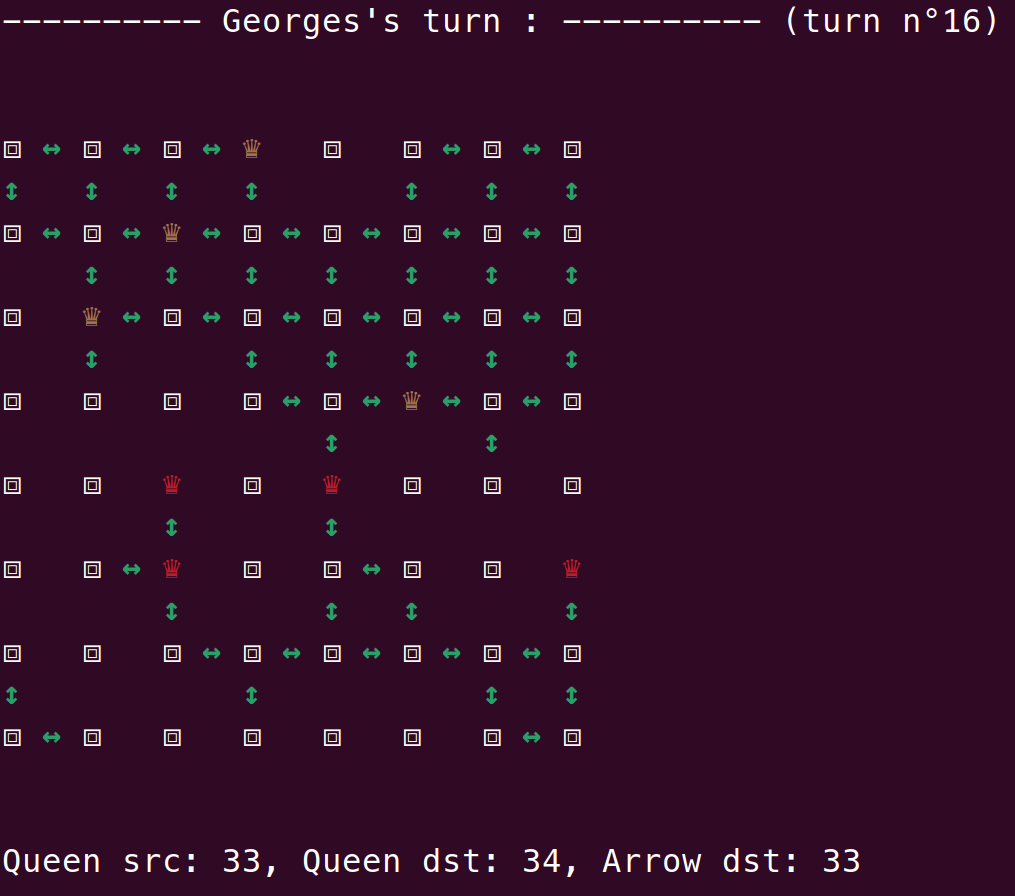
\includegraphics[width=10cm]{Capture d’écran du 2023-05-08 00-11-38.png}
    \caption{Exemple d'affichage pour un tour}
    \label{affi}
\end{figure}

\newpage
\section{Tests unitaires}
Lors de nos tests, nous avons majoritairement testé les fonctions communes aux deux joueurs et les fonctions qui sont utiles pour appliquer les règles de jeu, réaliser les mouvements ou encore mettre à jour le monde. Pour tester ces fonctions, nous avons réalisé des tests unitaires dans différentes situations afin de s'assurer que toutes les situations peuvent être traitées et que nos fonctions ne présentent pas de bugs. S'il y en a un, nous pouvons ainsi facilement le corriger. Les fonctions non testées sont les fonctions basiques et les fonctions d'affichage. En effet ces fonctions renvoient des résultats simples qui ne nécessitent pas d'être testées.

\vspace{1cm}
\section{Outils de travail}
Lors de ce projet, nous avons aussi eu l'occasion de continuer à améliorer notre utilisation de \textit{git} et des possibilités qu'il présente. Ainsi, nous n'avons pas hésité à créer des branches lorsque nous devions implémenter certaines fonctionnalités ou encore créer les stratégies des joueurs, l'utilisation de ces branches nous a permis de continuer à développer le projet en pouvant publier notre avancée sur la forge sans que cela affecte le code principal. Nous avons aussi pu utiliser \textbf{Valgrind} et \textbf{GDB} de manière plus efficace qu'au semestre précédent car nous avons appris quelques commandes supplémentaires.

\vspace{1cm}
\section{Conclusion}
Ce projet de programmation en équipe a été très instructif. En effet, il nous a permis de travailler nos compétences techniques en nous faisant aborder une autre vision de la programmation en C, avec notamment la gestion des visions serveur et client, l'importance des spécifications et une bonne gestion de la modularité. Mais ce n'est pas tout, en plus de ces compétences techniques, ce projet à 4 nous a aussi permis de travailler les compétences de travail en équipe comme la répartition des tâches, la mise en place d'échéances (qui sont vraiment essentielles pour avancer efficacement) et la gestion des egos et des idées, car savoir dialoguer sur une implémentation ou autre est la clé pour construire un projet cohérent. En conclusion, ce projet de programmation nous a permis de travailler des aspects importants de l'ingénieur informatique.

\end{document}